\chapter{Grundlagen}

In diesem Kapitel sollen einige grundlegenden Themen angesprochen werden, die dann im darauffolgenden Kapitel als bekannt vorausgesetzt werden. Dazu gehören zu einen Algorithmen, die in dieser Arbeit verwendet werden, aber nicht im Rahmen dieser entwickelt wurden. Zum anderen wird ein Überblick über das Framework gegeben, in das das entwickelte System eingebettet ist. Außerdem wird der Roboter an dem die Evaluation vorgenommen werden wird vorgestellt.

\section{Das ArmarX-Framework}
\subsection{Allgemeine Struktur und Funktionalitäten}

Das ArmarX-Framework ist ein sogenanntes \glqq Robot Development Environment\grqq{} (RDE). Ein Programm mit dem ohne viel Training des Benutzers und auf einem hohen Abstraktionsniveau Ansteuerungsprogramme für, in diesem Fall, humanoide Roboter erstellt werden können. Dieses Framework (\textcolor{red}{Referenz}) wird am Karlsruher Institut für Technologie (KIT) seit dem Jahr 2011 entwickelt und ist noch immer in der Weiterentwicklung. \\
Eine der Hauptaufgaben von RDEs ist dabei die Kommunikation zum einen zwischen der Hardware und der Software und zum anderen zwischen einzelnen Komponenten der Robotersteuerung. Hier wird dafür die Middleware \glqq Ice\grqq{} \textcolor{red}{Korrekter Name + Referenz} verwendet, die über das lokale Netzwerk erlaubt Komponenten auf verschiedenen Maschinen laufen zu lassen, die aber dennoch miteinander kommunizieren können. Das erlaubt eine bequeme Steuerung des Roboters von außerhalb: Die Lowlevel-Controller und die Hardware-Abstraktionen können auf den im Roboter verbauten PCs arbeiten, während auf einem externen PC rechenintensive Operationen wie Kinematik, Bildverarbeitung und die Highlevel-Robotersteuerung ausgeführt werden.
\\

ArmarX ist in drei Schichten unterteilt (vgl. Abb. \ref{fig:ArmarX_structure}): Zum Einen die bereits erwähnte Middleware-Schicht, die Funktionalitäten zur einfachen Erstellung von verteilten Anwendungen bietet. Außerdem das sogenannte \glqq Robot Framework Layer\grqq{}, welches grundlegende Funktionalitäten für die Robotersteuerung bereitstellt und schließlich die Anwendung-Schicht in der komplexe Roboterprogramme erstellt werden können.

\begin{figure}[h]
\begin{center}
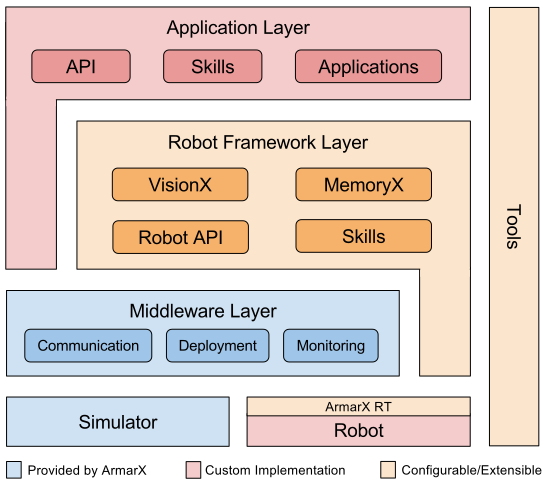
\includegraphics[width=0.7\textwidth]{ArmarX_Structure}
\caption{Fehlt}
\label{fig:ArmarX_structure}
\end{center}
\end{figure}

\paragraph{Middleware-Schicht} Jeder Programmbaustein in ArmarX ist eine Komponente, die einen geregelten Lebenszyklus hat. Zunächst wird die Komponente erstellt und dann auf mögliche Abhängigkeiten gewartet. Diese Abhängigkeiten sind in der Regel andere Komponenten die erst vollständig gestartet sein müssen, bevor die aktuelle Komponente selbst in den \textit{Gestartet}-Zustand übergehen kann. Falls eine Komponente im Laufe des Betriebs ausfällt, erkennt die Middleware-Schicht dies und bringt jede Komponente, die eine Abhängigkeit auf das fehlerhafte Objekt hat, in einen Wartezustand. Damit ist garantiert, dass zu keinem Zeitpunkt ein Methodenaufruf auf einem nicht korrekt laufenden Objekt getätigt wird. Somit wird verhindert, dass eine einzelne Komponente das gesamte Programm zum Absturz bringen kann.




\subsection{\textcolor{red}{Das Statechart-Konzept}}

\section{Der Humanoide Roboter ARMAR-IIIa}

\section{Inverse Kinematik}\label{sec:InverseKinematik}
\subsection{Constrained IK}\label{sec:ConstrainedIK}

\section{Bewegungsplanung} \label{sec:Bewegungsplanung}
\subsection{Rapidly-exploring random tree}

\section{Visual-Servoing}
\subsection{Objekterkennung}
\subsection{Objektverfolgung}